\documentclass[12pt,oneside,a4paper,chapter=TITLE]{abntex2}


\usepackage[T1]{fontenc}
\usepackage[utf8]{inputenc}
\usepackage[brazil]{babel}
\usepackage{indentfirst}
\usepackage{graphicx}
\usepackage{lmodern}



\titulo{FinControl: Desenvolvimento de Aplicação Web para Gestão Financeira Pessoal}

\autor{
Natan Gabriel de Souza Miranda \\
João Victor Soares de Lima \\
Kamilly Stephany Saraiva Santos \\
Samuel Alexandre Correia da Silva \\
Crytian Pinheiro Aguiar \\
Roberto Matheus Nunes dos Santos \\
Paulo Israel Pinho Filho
}

\instituicao{Centro Universitário Maurício de Nassau - UNINASSAU}
\local{Maceió - AL}
\data{2026}
\tipotrabalho{Relatório Técnico}

\begin{document}
\hypersetup{
    colorlinks=true,
    linkcolor=blue,
    citecolor=black,
    urlcolor=blue
}



\begin{figure}[h]
\centering

\includegraphics[width=4cm]{Logo_unina.png}
\end{figure}

\imprimircapa

\begin{folhaderosto}

\begin{center}


\includegraphics[width=4cm]{Logo_unina.png}

\vspace{2cm}

{\ABNTEXchapterfont\Large\imprimirautor}

\vfill

{\ABNTEXchapterfont\bfseries\LARGE\imprimirtitulo}

\vfill

\end{center}

\hspace*{8cm}
\begin{minipage}{8cm}
Trabalho apresentado à disciplina de Códigos de Alta Performance - Web do curso de Ciência da Computação do Centro Universitário Maurício de Nassau --- UNINASSAU, como requisito parcial para obtenção da nota da AV2.

\vspace{0.5cm}

Professor: Anderlan Henrique
\end{minipage}

\vfill

\begin{center}
\imprimirlocal

\imprimirdata
\end{center}

\end{folhaderosto}


\begin{resumo}
O presente trabalho apresenta o desenvolvimento do sistema FinControl, uma aplicação web voltada para a gestão financeira pessoal. O sistema foi concebido com o objetivo de auxiliar usuários no controle de receitas, despesas e metas financeiras, promovendo maior organização e clareza sobre sua situação econômica.

A aplicação foi desenvolvida utilizando React no frontend, aliado a bibliotecas modernas de visualização de dados como Recharts, além da utilização do JSON-Server para simulação de backend. O sistema permite o registro de transações financeiras, categorização de gastos, acompanhamento de metas e visualização de dashboards interativos.

O resultado final demonstra que a aplicação contribui significativamente para o controle financeiro pessoal, oferecendo uma interface intuitiva, responsiva e de fácil utilização.

\textbf{Palavras-chave}: Finanças pessoais. React. Dashboard. Gestão financeira. Aplicação web.
\end{resumo}

\tableofcontents*
\newpage


\textual

\chapter{Introdução}

A gestão financeira pessoal é um dos principais desafios enfrentados por indivíduos na sociedade contemporânea. O aumento do consumo digital, a facilidade de acesso ao crédito e a diversidade de formas de pagamento tornam o controle financeiro cada vez mais complexo.

Muitas pessoas enfrentam dificuldades em organizar suas receitas e despesas de forma eficiente, o que pode resultar em endividamento e falta de planejamento financeiro. Nesse contexto, soluções tecnológicas desempenham um papel fundamental na promoção de hábitos financeiros mais saudáveis.

O sistema FinControl foi desenvolvido com o objetivo de oferecer uma ferramenta acessível, moderna e intuitiva para auxiliar usuários na organização de suas finanças pessoais. A aplicação permite o registro detalhado de movimentações financeiras e apresenta visualizações gráficas que facilitam a compreensão dos dados.

Além disso, o sistema busca incentivar o planejamento financeiro por meio do acompanhamento de metas, proporcionando ao usuário uma visão clara de seus objetivos econômicos.


\section{Problema}

A principal problemática abordada neste trabalho refere-se à falta de controle financeiro por parte da população em geral. Grande parte dos usuários não possui ferramentas adequadas para acompanhar seus gastos de forma precisa e contínua.

O uso de métodos tradicionais, como anotações manuais ou planilhas simples, limita a capacidade de análise e não oferece recursos de automação ou visualização avançada de dados financeiros.


\section{Justificativa}

A criação do FinControl justifica-se pela necessidade de soluções tecnológicas mais acessíveis e eficientes para gestão financeira pessoal. A utilização de aplicações web permite acesso multiplataforma, facilitando o uso em diferentes dispositivos.

Além disso, a implementação de dashboards e gráficos interativos contribui para uma melhor interpretação dos dados, permitindo que o usuário tome decisões financeiras mais conscientes e fundamentadas.


\chapter{Objetivos}

\section{Objetivo Geral}

Desenvolver uma aplicação web para gestão financeira pessoal utilizando tecnologias modernas de desenvolvimento frontend.

\section{Objetivos Específicos}

\begin{itemize}
\item Desenvolver sistema de registro de receitas e despesas;
\item Implementar categorização de transações financeiras;
\item Criar dashboards interativos com gráficos;
\item Permitir acompanhamento de metas financeiras;
\item Aplicar conceitos de componentização em React;
\item Simular backend utilizando JSON-Server.
\end{itemize}


\chapter{Fundamentação Teórica}

O desenvolvimento de aplicações web modernas envolve o uso de tecnologias que permitem maior flexibilidade, escalabilidade e interatividade.

O React é uma das bibliotecas mais utilizadas atualmente no desenvolvimento frontend, sendo baseado em uma arquitetura de componentes reutilizáveis. Essa abordagem facilita a manutenção do código e melhora a organização do sistema.

A visualização de dados desempenha um papel fundamental em sistemas financeiros, pois permite transformar informações numéricas em representações gráficas de fácil interpretação. Ferramentas como o Recharts possibilitam a criação de gráficos dinâmicos que auxiliam o usuário na análise de seus gastos.

No contexto da gestão financeira pessoal, estudos indicam que a visualização clara de dados contribui para o aumento da consciência financeira e melhora o controle de gastos. Dessa forma, a tecnologia se torna uma aliada importante na educação financeira.


\chapter{Metodologia}

O desenvolvimento do sistema FinControl foi realizado por meio de uma abordagem incremental e modular.

A aplicação foi construída utilizando React, permitindo a criação de componentes independentes e reutilizáveis. Cada funcionalidade do sistema foi separada em módulos específicos, como receitas, despesas e metas financeiras.

Para simulação do backend, foi utilizado o JSON-Server, permitindo o armazenamento e manipulação de dados de forma simples durante o desenvolvimento.

Foram utilizados hooks do React para gerenciamento de estado, garantindo atualização dinâmica das informações na interface.

A arquitetura do sistema foi baseada em separação de responsabilidades, contribuindo para melhor organização e escalabilidade do código.


\chapter{Desenvolvimento do Sistema}

O sistema foi dividido em módulos principais:

\section{Módulo de Receitas}

Responsável pelo registro de entradas financeiras, como salários e rendimentos diversos. O módulo permite categorização e visualização das receitas cadastradas.

\section{Módulo de Despesas}

Permite o controle detalhado de gastos, incluindo valor, categoria, data e forma de pagamento. Esse módulo auxilia o usuário a identificar padrões de consumo.

\section{Módulo de Metas}

Permite a criação e acompanhamento de objetivos financeiros, apresentando progresso percentual baseado nos valores acumulados.

\section{Dashboard}

O dashboard apresenta uma visão geral da situação financeira do usuário, utilizando gráficos e indicadores para facilitar a análise.


\chapter{Resultados e Discussão}

O sistema desenvolvido apresentou resultados satisfatórios em relação aos objetivos propostos.

A interface demonstrou ser intuitiva e de fácil utilização, permitindo que o usuário registre e acompanhe suas finanças de forma clara.

\begin{figure}[h]
\centering
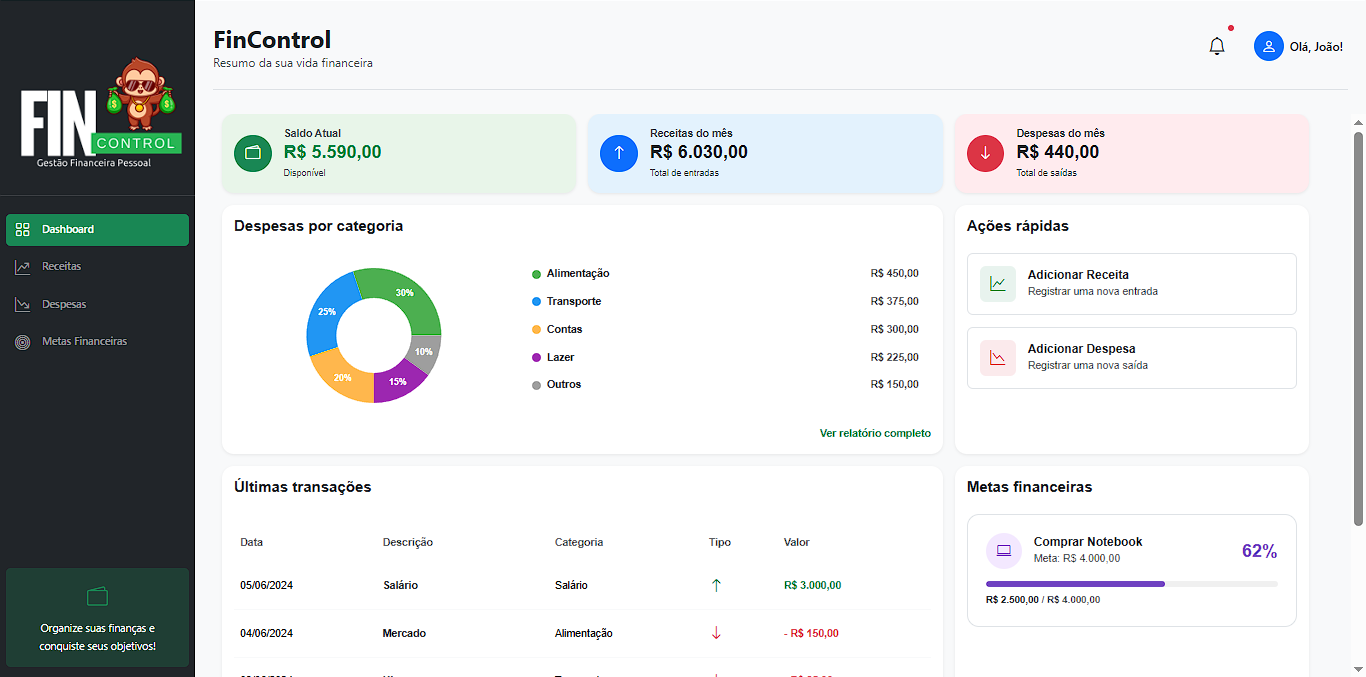
\includegraphics[width=0.95\textwidth]{Projeto_unina.png}
\caption{Tela principal do sistema FinControl}
\label{fig:fincontrol}
\end{figure}

A utilização de gráficos contribuiu significativamente para a visualização dos dados, tornando mais fácil a compreensão dos padrões de gastos.

O módulo de metas mostrou-se eficiente no incentivo ao planejamento financeiro, permitindo ao usuário acompanhar seu progresso de forma visual e motivadora.

\chapter{Conclusão}

Conclui-se que o sistema FinControl atende de forma eficaz à proposta de oferecer uma ferramenta de gestão financeira pessoal.

A aplicação demonstra a importância do uso de tecnologias web modernas no desenvolvimento de soluções práticas para problemas do cotidiano.

Como trabalhos futuros, sugere-se a integração com APIs bancárias reais, implementação de autenticação de usuários e armazenamento em nuvem, ampliando a funcionalidade e escalabilidade do sistema.


\chapter*{Referências}

REACT. React Documentation. Disponível em: https://react.dev

BOOTSTRAP. Bootstrap Documentation. Disponível em: https://getbootstrap.com

RECHARTS. Recharts Documentation. Disponível em: https://recharts.org

NODE.JS. Node.js Documentation. Disponível em: https://nodejs.org

JSON-SERVER. JSON Server Documentation. Disponível em: https://github.com/typicode/json-server

BOOTSTRAP ICONS. Documentation. Disponível em: https://icons.getbootstrap.com

VISUAL STUDIO CODE. Documentation. Disponível em: https://code.visualstudio.com

\end{document}